
\lecture{Correlation and Regression}{correlation-regression}
\section{Correlation and Regression}

\title{Correlation and Linear Regression}
\subtitle{Is a Straight Line Appropriate?}

%\author{Kelly Black}
%\institute{Clarkson University}
\date{25 January 2012}

\begin{frame}
  \titlepage
\end{frame}

\begin{frame}
  \frametitle{Outline}
  \tableofcontents[pausesection,hideothersubsections,sectionstyle=show/hide]
\end{frame}


\subsection{Clicker Quiz}


\begin{frame}{Clicker Quiz}

Determine if the following relationship is a ``positive relationship''
or a ``negative relationship'' between the two variables.

\begin{center}
  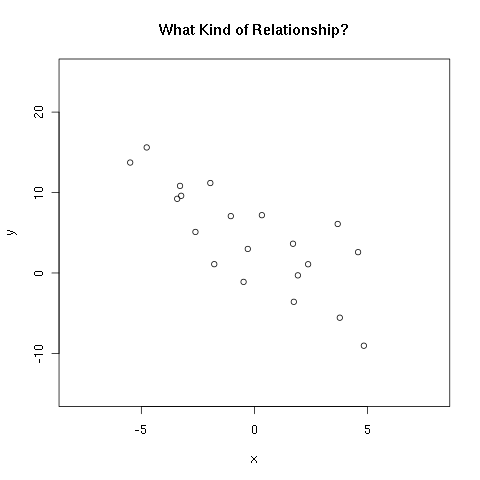
\includegraphics[width=6cm]{img/week2Day3ClickerQuizNeg}
\end{center}

\begin{tabular}{l@{\hspace{3em}}l}
  A: Positive & B: Negative
\end{tabular}


\end{frame}


\begin{frame}{Positive vs. Negative Relationships}

  \begin{columns}
    \column{.5\textwidth}
    Positive Relationship: \\
    \centerline{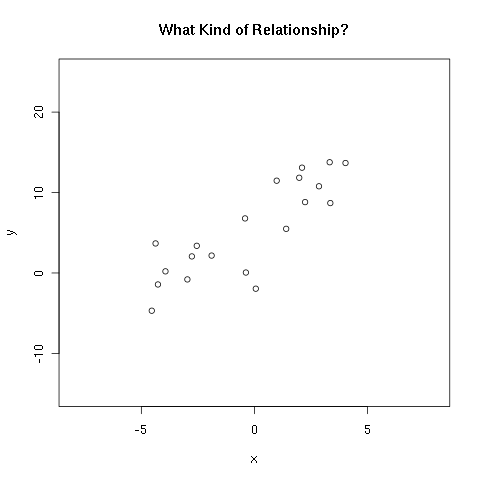
\includegraphics[width=5cm]{img/week2Day3ClickerQuizPos}}
    \column{.5\textwidth}
    Negative Relationship: \\
    \centerline{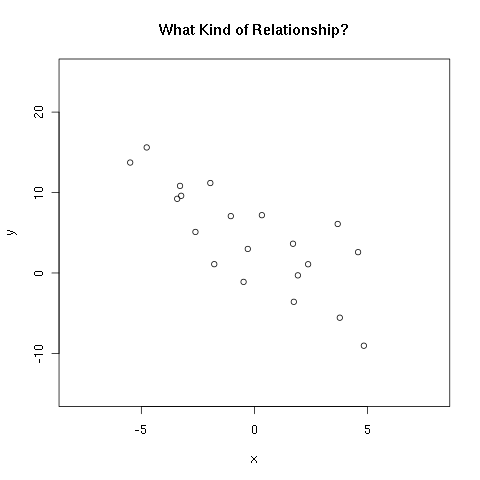
\includegraphics[width=5cm]{img/week2Day3ClickerQuizNeg}}
  \end{columns}
  
\end{frame}



\subsection{Correlation}

\begin{frame}{Correlation}

  \hspace*{-3em}
  \begin{tabular}{rrr}
    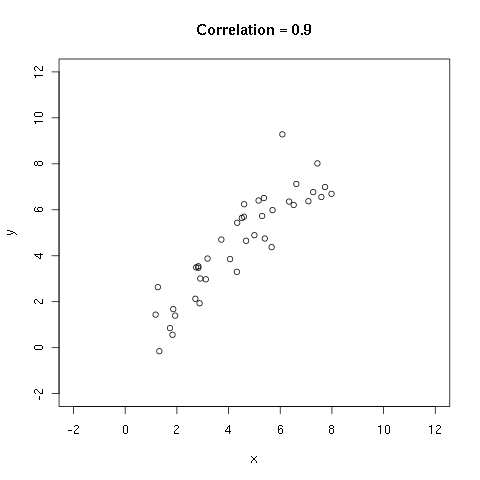
\includegraphics[height=4cm]{img/correlation09} & 
    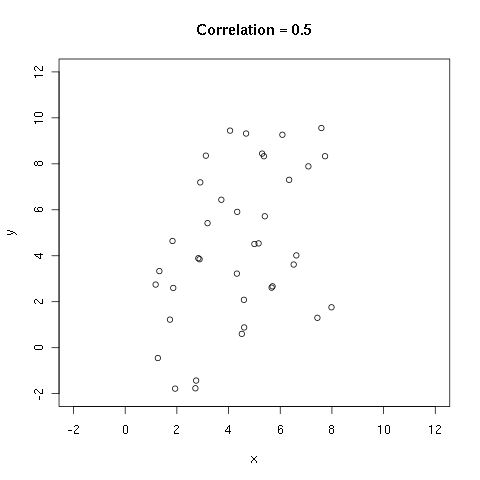
\includegraphics[height=4cm]{img/correlation05} &
    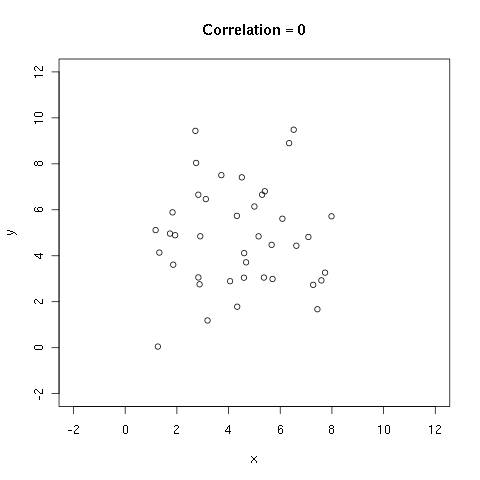
\includegraphics[height=4cm]{img/correlation0} \\
    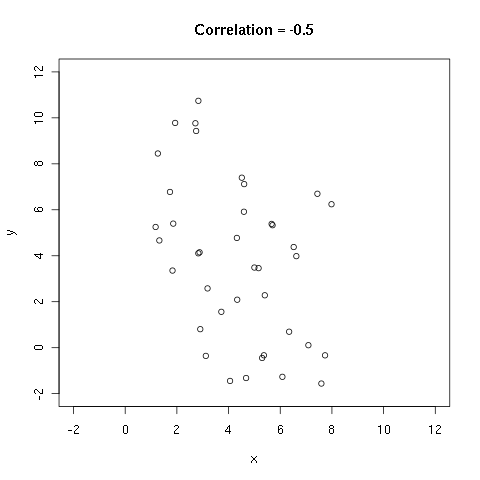
\includegraphics[height=4cm]{img/correlation-05} &
    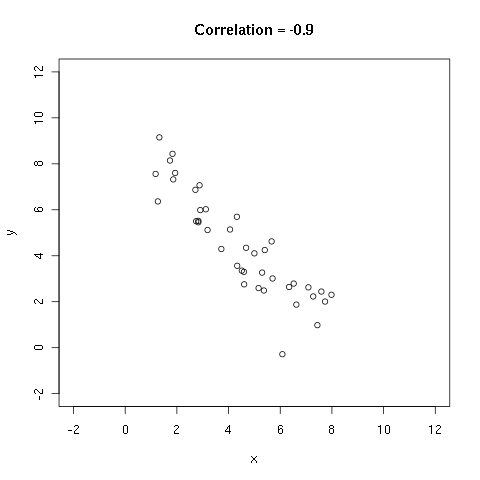
\includegraphics[height=4cm]{img/correlation-09}
  \end{tabular}


\end{frame}


\begin{frame}{Calculating the Correlation}

  First define the following sums:
  \begin{eqnarray*}
    S_{xx} & = & (x_1-\bar{x})^2 + (x_2-\bar{x})^2 + \cdot + (x_n-\bar{x})^2, \\
    S_{yy} & = & (y_1-\bar{y})^2 + (y_2-\bar{y})^2 + \cdot + (y_n-\bar{y})^2, \\
    S_{xy} & = & (x_1-\bar{x}) + (x_2-\bar{x}) + \cdot + (x_n-\bar{x}), \\
  \end{eqnarray*}

  \uncover<2->
  {
    
    \begin{definition}
      The sample correlation coefficient is defined to be
      \begin{eqnarray*}
        r & = & \frac{S_{xy}}{\sqrt{S_{xx} S_{yy}}}.
      \end{eqnarray*}
    \end{definition}

  }
  
\end{frame}



\begin{frame}{Example}
  
  \begin{columns}
    \column{.25\textwidth}
    \begin{tabular}{l|l}
      $x$ & $y$ \\ \hline
      -1 & -1 \\
      0 & 1 \\
      1 & 2 \\
      2 & 4
    \end{tabular}

    \column{.75\textwidth}
    
    \uncover<2->
    {
      \centerline{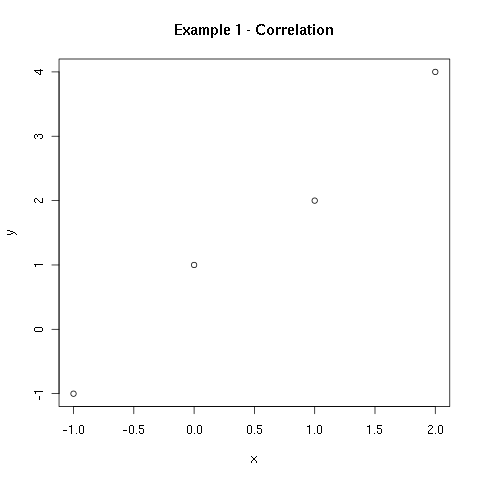
\includegraphics[width=6cm]{img/week2-Day3Correlation}}
    }

    \end{columns}

\end{frame}


\subsection{Linear Regression}


\begin{frame}{Clicker Quiz 2}
  
  \begin{columns}
    \column{.25\textwidth}
    \begin{tabular}{l|l}
      $x$ & $y$ \\ \hline
      -1 & -1 \\
      0 & 1 \\
      1 & 2 \\
      2 & 4
    \end{tabular}

    \column{.75\textwidth}

    What is $S_{yy}$?

    \begin{tabular}{l@{\hspace{3em}}l@{\hspace{3em}}l}
      A: 5  & B: 8.5 & C: 16.75
    \end{tabular}


    \end{columns}

\end{frame}


\begin{frame}{Example}
  
  \begin{columns}
    \column{.25\textwidth}
    \begin{tabular}{l|l}
      $x$ & $y$ \\ \hline
      -1 & -1 \\
      0 & 1 \\
      1 & 2 \\
      2 & 4
    \end{tabular}

    \column{.75\textwidth}
    
    \only<2>
    {
      \centerline{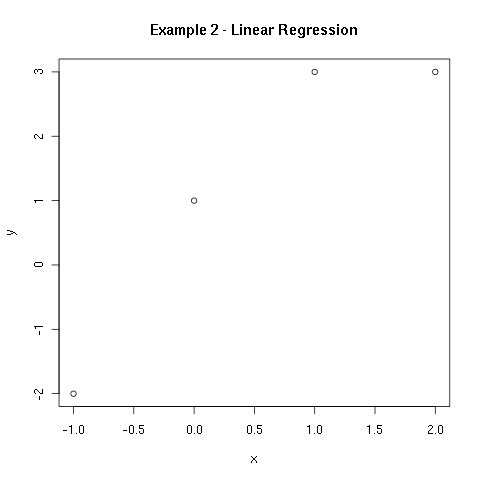
\includegraphics[width=6cm]{img/week2-Day3-Regression1}}
    }

    \only<3>
    {
      \centerline{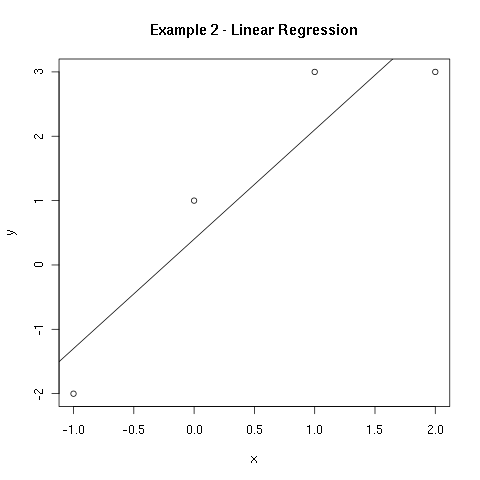
\includegraphics[width=6cm]{img/week2-Day3-Regression2}}
    }


    \end{columns}

\end{frame}




% LocalWords:  Clarkson pausesection hideallsubsections rrr yy xy
